\documentclass[a4paper,14pt]{extarticle}

\usepackage[utf8x]{inputenc}
\usepackage[T1,T2A]{fontenc}
\usepackage[russian]{babel}
\usepackage{hyperref}
\usepackage{indentfirst}
\usepackage{here}
\usepackage{array}
\usepackage{graphicx}
\usepackage{caption}
\usepackage{subcaption}
\usepackage{chngcntr}
\usepackage{amsmath}
\usepackage{amssymb}
\usepackage{pgfplots}
\usepackage{pgfplotstable}
\usepackage[left=2cm,right=2cm,top=2cm,bottom=2cm,bindingoffset=0cm]{geometry}
\usepackage{multicol}
\usepackage{askmaps}
\usepackage{titlesec}
\usepackage{listings}
\usepackage{color}
\usepackage{courier}

\definecolor{green}{rgb}{0,0.6,0}
\definecolor{gray}{rgb}{0.5,0.5,0.5}
\definecolor{purple}{rgb}{0.58,0,0.82}

\lstset{
	language=Verilog,
	backgroundcolor=\color{white},   
	basicstyle=\small\ttfamily,
	commentstyle=\color{green},
	keywordstyle=\color{blue},	
	numberstyle=\tiny\color{gray},
	stringstyle=\color{purple},
	breakatwhitespace=false,
	breaklines=true,
	captionpos=b,
	keepspaces=true,
	numbers=left,
	numbersep=5pt,
	showspaces=false,
	showstringspaces=false,
	showtabs=false,
	tabsize=4,
	frame=single,
	inputpath={../quartus/},
	literate={~} {$\sim$}{1}
}

\renewcommand{\le}{\ensuremath{\leqslant}}
\renewcommand{\leq}{\ensuremath{\leqslant}}
\renewcommand{\ge}{\ensuremath{\geqslant}}
\renewcommand{\geq}{\ensuremath{\geqslant}}
\renewcommand{\epsilon}{\ensuremath{\varepsilon}}
\renewcommand{\phi}{\ensuremath{\varphi}}
\renewcommand{\thefigure}{\arabic{figure}} 	
\renewcommand*\not[1]{\overline{#1}}

\titleformat*{\section}{\large\bfseries} 
\titleformat*{\subsection}{\normalsize\bfseries} 
\titleformat*{\subsubsection}{\normalsize\bfseries} 
\titleformat*{\paragraph}{\normalsize\bfseries} 
\titleformat*{\subparagraph}{\normalsize\bfseries} 

\counterwithin{figure}{section}
\counterwithin{equation}{section}
\counterwithin{table}{section}
\newcommand{\sign}[1][5cm]{\makebox[#1]{\hrulefill}}
\graphicspath{{../pics/}}
\captionsetup{justification=centering,margin=1cm}
\def\arraystretch{1.3}
\setlength\parindent{5ex}
\titlelabel{\thetitle.\quad}

\begin{document}

\begin{titlepage}
\begin{center}
	Санкт-Петербургский Политехнический Университет Петра Великого\\[0.3cm]
	Институт компьютерных наук и технологий \\[0.3cm]
	Кафедра компьютерных систем и программных технологий\\[4cm]
	
	\textbf{ОТЧЕТ}\\ 
	\textbf{по лабораторной работе}\\[0.5cm]
	\textbf{SystemVerilog №4}\\[0.1cm]
	Автоматизация проектирования\\ дискретных устройств\\[4.0cm]
\end{center}

\begin{flushright}
	\begin{minipage}{0.45\textwidth}
		\textbf{Работу выполнил студент}\\[3mm]
		группа 33501/4 \hspace*{9mm} Дьячков В.В.\\[5mm]
		\textbf{Преподаватель}\\[5mm]
		\sign[1.5cm] \hspace*{1mm} к.т.н., доц. Филиппов А.С. \\[5mm]
	\end{minipage}
\end{flushright}

\vfill

\begin{center}
	Санкт-Петербург\\
	\the\year
\end{center}
\end{titlepage}

\addtocounter{page}{1}
\counterwithin{lstlisting}{section}

\tableofcontents
%\newpage
\listoffigures
\lstlistoflistings
\newpage

\section{lab2\_1}

\subsection{Задание}

На языке Verilog опишите знаковый сумматор:
\begin{itemize}
	\item Входы данных переключатели \code{sw[7:4]} и \code{sw[3:0]} соответственно.
	\item Выходы – светодиоды \code{led[4:0]}.
\end{itemize}

В описании можно использовать любые операторы. Тип данных - \code{wire}.

\subsection{Код на языке Verilog}

В листинге \ref{code:1} приведен код программы на языке Verilog.

\lstinputlisting[caption=lab2\_1.v, label=code:1]{lab2_1/lab2_1.v}

\subsection{Результаты синтеза}

На рис. \ref{fig:lab2_1_rtl} приведено изображение синтезированной схемы в RLT Viewer.

\begin{figure}[H]
\begin{center}
	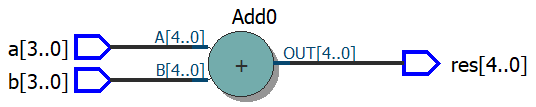
\includegraphics[scale=0.7]{lab2_1_rtl}
	\caption{Результат синтеза в RLT Viewer}
	\label{fig:lab2_1_rtl}
\end{center}
\end{figure}

\subsection{Результаты моделирования}
\label{sec:lab2_1_modeling}

На рис. \ref{fig:lab2_1_modeling} изображена временная диаграмма работы синтезированного устройства. На вход устройству поочередно подаются случайные знаковые значения \code{a[3:0]} и \code{b[3:0]}, а результат записывается в \code{res[4:0]}.
\begin{figure}[H]
\begin{center}
	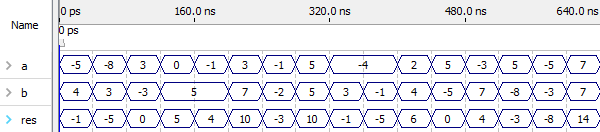
\includegraphics[width=\textwidth]{lab2_1_modeling}
	\caption{Результаты моделирования}
	\label{fig:lab2_1_modeling}
\end{center}
\end{figure}

\subsection{Назначение выводов СБИС}

На рис. \ref{fig:lab2_1_pins} приведены назначения выводов СБИС в Pin Planner.

\begin{figure}[H]
\begin{center}
	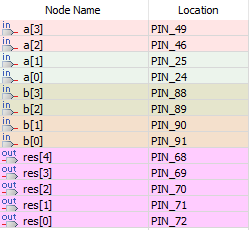
\includegraphics{lab2_1_pins}
	\caption{Таблица назначений в Pin Planer}
	\label{fig:lab2_1_pins}
\end{center}
\end{figure}

\subsection{Результаты проверки на плате}

Для тестирования проекта на плате были использованы тесты, описанные в пункте \ref{sec:lab2_1_modeling}. Результаты тестирования совпадают с ожидаемыми, следовательно, устройство работает верно.

\subsection{Выводы}

Разработан знаковый сумматор. Результаты моделирования и тестирования на плате показали, что разработанное устройство работает верно.

\newpage

\section{lab2\_2}

\subsection{Задание}

На языке Verilog опишите знаковый умножитель:
\begin{itemize}
	\item Входы данных переключатели \code{sw[7:4]} и \code{sw[3:0]} соответственно.
	\item Выходы – светодиоды \code{led[4:0]}.
\end{itemize}

В описании можно использовать любые операторы. Тип данных - \code{wire}.

\subsection{Код на языке Verilog}

В листинге \ref{code:2} приведен код программы на языке Verilog.

\lstinputlisting[caption=lab2\_2.v, label=code:2]{lab2_2/lab2_2.v}

\subsection{Результаты синтеза}

На рис. \ref{fig:lab2_2_rtl} приведено изображение синтезированной схемы в RLT Viewer.

\begin{figure}[H]
\begin{center}
	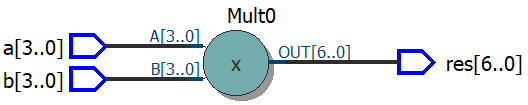
\includegraphics[scale=0.7]{lab2_2_rtl}
	\caption{Результат синтеза в RLT Viewer}
	\label{fig:lab2_2_rtl}
\end{center}
\end{figure}

\subsection{Результаты моделирования}
\label{sec:lab1_2_modeling}

На рис. \ref{fig:lab2_2_modeling} изображена временная диаграмма работы синтезированного устройства. На вход устройству поочередно подаются случайные знаковые значения \code{a[3:0]} и \code{b[3:0]}, а результат записывается в \code{res[6:0]}.
\begin{figure}[H]
\begin{center}
	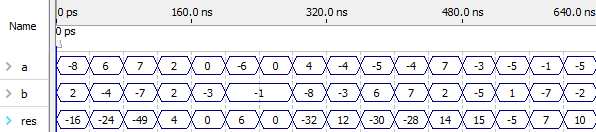
\includegraphics[width=\textwidth]{lab2_2_modeling}
	\caption{Результаты моделирования}
	\label{fig:lab2_2_modeling}
\end{center}
\end{figure}

\subsection{Назначение выводов СБИС}

На рис. \ref{fig:lab2_2_pins} приведены назначения выводов СБИС в Pin Planner.

\begin{figure}[H]
\begin{center}
	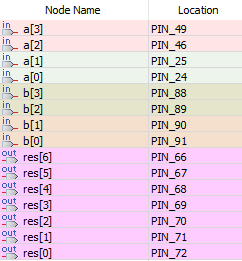
\includegraphics{lab2_2_pins}
	\caption{Таблица назначений в Pin Planer}
	\label{fig:lab2_2_pins}
\end{center}
\end{figure}

\subsection{Результаты проверки на плате}

Для тестирования проекта на плате были использованы тесты, описанные в пункте \ref{sec:lab1_2_modeling}. Результаты тестирования совпадают с ожидаемыми, следовательно, устройство работает верно.

\subsection{Выводы}

Разработан знаковый умножитель. Результаты моделирования и тестирования на плате показали, что разработанное устройство работает верно.

\newpage

\section{lab2\_3}

\subsection{Задание}

На языке Verilog опишите без знаковый делитель с формированием остатка от деления:
\begin{itemize}
\item Входы
	\begin{itemize}
		\item Делимое -- переключатели \code{sw[7:4]};
		\item Делитель -- переключатели \code{sw[3:0]}.
	\end{itemize}
\item Выходы
	\begin{itemize}
		\item Результат деления -- светодиоды \code{led[7:4]};
		\item Остаток от деления -- светодиоды \code{led[3:0]}.
	\end{itemize}
\end{itemize}

В описании можно использовать любые операторы. Тип данных - \code{wire}.

\subsection{Код на языке Verilog}

В листинге \ref{code:3} приведен код программы на языке Verilog.

\lstinputlisting[caption=lab2\_3.v, label=code:3]{lab2_3/lab2_3.v}

\subsection{Результаты синтеза}

На рис. \ref{fig:lab2_3_rtl} приведено изображение синтезированной схемы в RLT Viewer.

\begin{figure}[H]
\begin{center}
	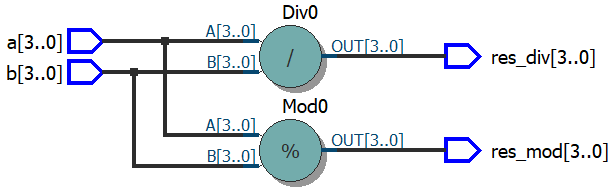
\includegraphics[scale=0.7]{lab2_3_rtl}
	\caption{Результат синтеза в RLT Viewer}
	\label{fig:lab2_3_rtl}
\end{center}
\end{figure}

\subsection{Результаты моделирования}
\label{sec:lab2_3_modeling}

На рис. \ref{fig:lab2_3_modeling} изображена временная диаграмма работы синтезированного устройства. На вход устройству поочередно подаются случайные без знаковые значения \code{a[3:0]} и \code{b[3:0]}, результат деления записывается в \code{res_div[3:0]}, а остаток от деления в \code{res_mod[3:0]}.
\begin{figure}[H]
\begin{center}
	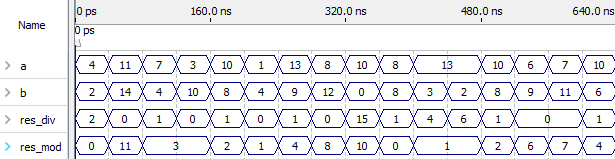
\includegraphics[width=\textwidth]{lab2_3_modeling}
	\caption{Результаты моделирования}
	\label{fig:lab2_3_modeling}
\end{center}
\end{figure}

\subsection{Назначение выводов СБИС}

На рис. \ref{fig:lab2_3_pins} приведены назначения выводов СБИС в Pin Planner.

\begin{figure}[H]
\begin{center}
	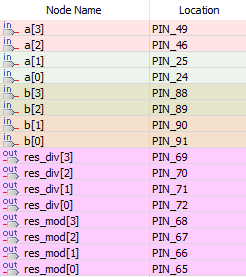
\includegraphics{lab2_3_pins}
	\caption{Таблица назначений в Pin Planer}
	\label{fig:lab2_3_pins}
\end{center}
\end{figure}

\subsection{Результаты проверки на плате}

Для тестирования проекта на плате были использованы тесты, описанные в пункте \ref{sec:lab2_3_modeling}. Результаты тестирования совпадают с ожидаемыми, следовательно, устройство работает верно.

\subsection{Выводы}

Разработан без знаковый делитель с формирование остатка от деления.  Результаты моделирования и тестирования на плате показали, что разработанное устройство работает верно.


\section{lab2\_4}

\subsection{Задание}

На языке Verilog опишите устройство возведения без знакового числа в фиксированную степень (степень без знака):
\begin{itemize}
	\item Значение степени равно 3.
	\item Входы данных переключатели \code{sw[1:0]} соответственно.
	\item Выходы – светодиоды \code{led[5:0]}.
\end{itemize}

В описании можно использовать любые операторы. Тип данных - \code{wire}.

\subsection{Код на языке Verilog}

В листинге \ref{code:4} приведен код программы на языке Verilog.

\lstinputlisting[caption=lab2\_4.v, label=code:4]{lab2_4/lab2_4.v}

\subsection{Результаты синтеза}

На рис. \ref{fig:lab2_4_rtl} приведено изображение синтезированной схемы в RLT Viewer.

\begin{figure}[H]
\begin{center}
	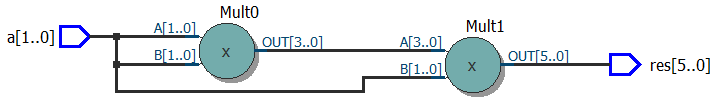
\includegraphics[scale=0.8]{lab2_4_rtl}
	\caption{Результат синтеза в RLT Viewer}
	\label{fig:lab2_4_rtl}
\end{center}
\end{figure}

\subsection{Результаты моделирования}
\label{sec:lab2_4_modeling}

На рис. \ref{fig:lab2_4_modeling} изображена временная диаграмма работы синтезированного устройства. На вход устройству поочередно подаются случайные без знаковые значения \code{a[1:0]}, а результат возведения в степень записывается в \code{res[5:0]}.
\begin{figure}[H]
\begin{center}
	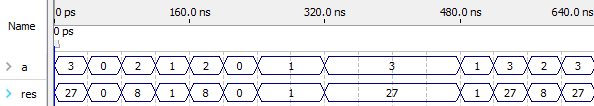
\includegraphics[width=\textwidth]{lab2_4_modeling}
	\caption{Результаты моделирования}
	\label{fig:lab2_4_modeling}
\end{center}
\end{figure}

\subsection{Назначение выводов СБИС}

На рис. \ref{fig:lab2_4_pins} приведены назначения выводов СБИС в Pin Planner.

\begin{figure}[H]
\begin{center}
	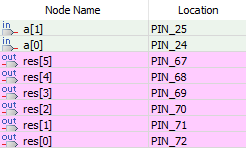
\includegraphics{lab2_4_pins}
	\caption{Таблица назначений в Pin Planer}
	\label{fig:lab2_4_pins}
\end{center}
\end{figure}

\subsection{Результаты проверки на плате}

Для тестирования проекта на плате были использованы тесты, описанные в пункте \ref{sec:lab2_4_modeling}. Результаты тестирования совпадают с ожидаемыми, следовательно, устройство работает верно.

\subsection{Выводы}

Разработано устройство возведения в степень. Результаты моделирования и тестирования на плате показали, что разработанное устройство работает верно.

\newpage

\section{elab2\_1}

\subsection{Задание}

На языке Verilog опишите без знаковый делитель с повышенной точностью (4 знака после запятой):
\begin{itemize}
\item Входы
	\begin{itemize}
		\item Делимое - переключатели \code{sw[7:4]};
		\item Делитель - переключатели \code{sw[3:0]}.
	\end{itemize}
\item Выходы
	\begin{itemize}
		\item Результат деления - светодиоды \code{led[7:4]};
		\item Знаки после запятой – светодиоды \code{led[3:0]}.
	\end{itemize}
\end{itemize}

В описании можно использовать любые операторы. Тип данных - \code{wire}.

\subsection{Код на языке Verilog}

В листинге \ref{code:5} приведен код программы на языке Verilog.

\lstinputlisting[caption=elab2\_1.v, label=code:5]{elab2_1/elab2_1.v}

\subsection{Результаты синтеза}

На рис. \ref{fig:elab2_1_rtl} приведено изображение синтезированной схемы в RLT Viewer.

\begin{figure}[H]
\begin{center}
	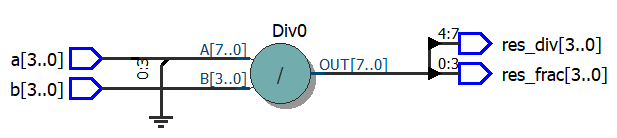
\includegraphics[scale=0.8]{elab2_1_rtl}
	\caption{Результат синтеза в RLT Viewer}
	\label{fig:elab2_1_rtl}
\end{center}
\end{figure}

\subsection{Результаты моделирования}
\label{sec:elab2_1_modeling}

На рис. \ref{fig:elab2_1_modeling} изображена временная диаграмма работы синтезированного устройства. На вход устройству поочередно подаются случайные без знаковые значения \code{a[3:0]} и \code{b[3:0]}, результат деления записывается в \code{res_div[3:0]}, а знаки после запятой в \code{res_frac[3:0]}.
\begin{figure}[H]
\begin{center}
	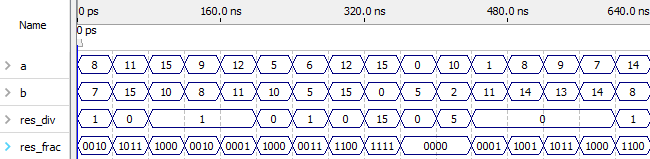
\includegraphics[width=\textwidth]{elab2_1_modeling}
	\caption{Результаты моделирования}
	\label{fig:elab2_1_modeling}
\end{center}
\end{figure}

\subsection{Назначение выводов СБИС}

На рис. \ref{fig:elab2_1_pins} приведены назначения выводов СБИС в Pin Planner.

\begin{figure}[H]
\begin{center}
	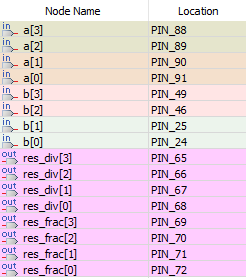
\includegraphics{elab2_1_pins}
	\caption{Таблица назначений в Pin Planer}
	\label{fig:elab2_1_pins}
\end{center}
\end{figure}

\subsection{Результаты проверки на плате}

Для тестирования проекта на плате были использованы тесты, описанные в пункте \ref{sec:elab2_1_modeling}. Результаты тестирования совпадают с ожидаемыми, следовательно, устройство работает верно.

\subsection{Выводы}

Разработан без знаковый делитель с повышенной точностью. Результаты моделирования и тестирования на плате показали, что разработанное устройство работает верно.

\section{elab2\_2}

\subsection{Задание}

\noindent На языке Verilog опишите знаковый умножитель на фиксированное число:
\begin{itemize}
	\item Множитель равен 9.
	\item Входы данных - переключатели \code{sw[3:0]} соответственно.
	\item Выходы – светодиоды \code{led[7:0]}.
\end{itemize}

\noindent В описании можно использовать операторы сдвига, сложения, вычитания, Replicator, Concatenate.

\subsection{Код на языке Verilog}

В листинге \ref{code:6} приведен код программы на языке Verilog.

\lstinputlisting[caption=elab2\_2.v, label=code:6]{elab2_2/elab2_2.v}

\subsection{Результаты синтеза}

На рис. \ref{fig:elab2_2_rtl} приведено изображение синтезированной схемы в RLT Viewer.

\begin{figure}[H]
\begin{center}
	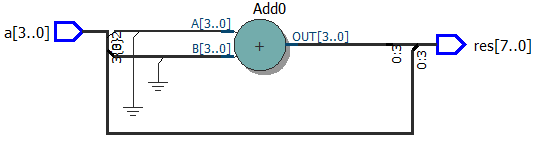
\includegraphics[scale=0.9]{elab2_2_rtl}
	\caption{Результат синтеза в RLT Viewer}
	\label{fig:elab2_2_rtl}
\end{center}
\end{figure}

\subsection{Результаты моделирования}
\label{sec:elab2_2_modeling}

На рис. \ref{fig:elab2_2_modeling} изображена временная диаграмма работы синтезированного устройства. На вход устройству поочередно подаются случайное знаковое значение \code{a[3:0]}, а результат умножения записывается в \code{res[7:0]}.

\begin{figure}[H]
\begin{center}
	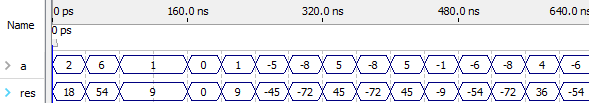
\includegraphics[width=\textwidth]{elab2_2_modeling}
	\caption{Результаты моделирования}
	\label{fig:elab2_2_modeling}
\end{center}
\end{figure}

\subsection{Назначение выводов СБИС}

На рис. \ref{fig:elab2_2_pins} приведены назначения выводов СБИС в Pin Planner.

\begin{figure}[H]
\begin{center}
	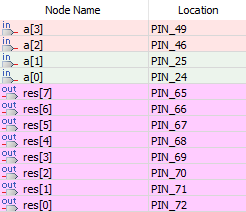
\includegraphics{elab2_2_pins}
	\caption{Таблица назначений в Pin Planer}
	\label{fig:elab2_2_pins}
\end{center}
\end{figure}

\subsection{Результаты проверки на плате}

Для тестирования проекта на плате были использованы тесты, описанные в пункте \ref{sec:elab2_2_modeling}. Результаты тестирования совпадают с ожидаемыми, следовательно, устройство работает верно.

\subsection{Выводы}

Разработан знаковый умножитель на фиксированное число. Результаты моделирования и тестирования на плате показали, что разработанное устройство работает верно.

\end{document}